% status: 100
% chapter: Blockchain

\title{Openchain}


\author{Stephen Giuliani}
\affiliation{%
  \institution{Indiana University}
  \state{Virginia}
  \country{USA}
}
\email{sgiulian@umail.iu.edu}

\renewcommand{\shortauthors}{S. Giuliani}

\begin{abstract}
Openchain is an open source blockchain technology developed so that enterprises
could stand up their own, fully functional, secure, highly customizable,
blockchain environment while maintaining full administration rights beginning
with the transactions recorded on the chain themselves through the validation
processes and even how the data is stored and used.
\end{abstract}

\keywords{hid-sp18-507, Openchain, Blockchain, Bitcoin, Open Source}

\maketitle

\section{Introduction}
Openchain is a blockchain technology designed as a simple yet customizable,
enterprise-ready, cryptographic ledger to track the ownership of digital and
real-world assets. Openchain offers both the back-end blockchain framework as
well as a blockchain-enabled wallet for managing digital assets. The open
source technology company leverages its online development community and offers
support in designing and building a blockchain network for client-specific
needs. Openchain's design differs from other and more traditional blockchain
concepts by utilizing a client-designed hierarchy for validating assets and
transactions, rather than using an anonymous decentralized validation system.
Openchain's blockchain concept can be stood-up in seconds and is fully
customizable for any individual's, company's, or asset-type's needs and the
open-source nature ensures constant development and improvements.

\section{Blockchain}
In recent years, the concept of blockchain has established itself as a
promising innovative technology with profitable, real-world implications and
interest in blockchain technologies peaked in late 2017. But what is
`Blockchain' and what does this technology mean for existing industries? In
order to understand the capabilities and near-future potential impacts this
technology will have on the world, we mist first understand what it is. Running
a basic search on the web for `Blockchain' is sure to turn up resulting
descriptions that use the terms `distributed ledger', `decentralized', and
`transparent'. Blockchain is a distributed ledger meaning that the data records
(ledger) is duplicated and maintained on any number of computers or servers
worldwide (distributed). The idea behind the distributed ledger is security in
the sense that the data records must be identical across all servers so that
any discrepancies, errors, or attempts to change information will be virtually
impossible to occur. The concept of verifying information and ensuring no foul
play or errors occurred exists in many industries today but the process of
guaranteeing the information is accurate is precisely what Blockchain
technology is designed to tackle. A prime example is how banking institutions
verify account balances and the ability to transfer money or pay for goods and
services. A bank would have to verify the originating account's balance to
ensure sufficient funds are available prior to the transaction. Then the bank
would verify the address or location of the destination account; sometimes,
this is a different banking institution with similar processes. Finally, once
the transaction is completed, all parties must verify completion and maintain
records of that transaction for any auditing purposes. Blockchain is expected
to disrupt this process, and many similar in concept, by cutting out the middle
man, or in this case, the banks. Through the use of a blockchain, the account
balance, address, destination address and balance are all connected on the same
chain through information in some form or another. This information is stored
as blocks, or essentially a collective of information making up some defined
amount of memory, which are all connected (block-chain) and therefore can be
verified through a query rather than (sometimes multiple) a middle-man like a
bank. Financial transactions and institutions are not the only industry
threatened by the use of blockchain technology. FUTURETHINKERS, a popular
podcast covering evolving technologies, discusses 19 major industries that will
likely be impacted by blockchain technology in a big way~\cite{FutureThinkers}.
Any institution who's responsibility is to verify or maintain ownership of an
asset can be disrupted by the adoption of blockchain; however many of these
institutions are recognizing the potential of blockchain technology and have
begun investing in utilizing the technology themselves. 

Understanding the distributed-ledger concept is only half of the defining
capability within a blockchain. Blockchains are, by design, secure through the
use of various cryptography practices. Blockchain technology utilizes
cryptography and dual-pair public and private keys to verify the users of the
chain itself. The information stored within the blocks of a blockchain is
transparent so that anyone with access to the chain can view the information
stored on the chain; however only the owner of the private key can make changes
(depending on the chain, such as a transaction) to their account. This
description is very high-level and the blockchain technologies in use today
invoke a wide variety of characteristics that make each unique. Blocks can vary
in size, enabling less or more information stored per block and entry within a
block. The ability to view, add, or change the information within a blockchain
can be enabled or disabled by the administer of the blockchain. And the purpose
of the blockchain can vary from any need to store information securely.

Most notably in today's media, cryptocurrency is at the forefront of blockchain
use and is the driving force behind its adoption as well as its hype. According
to Google trends, the idea of cryptocurrency spiked interest far beyond
blockchain, the technology behind cryptocurrency, tokens, and initial coin
offerings, or ICOs (see Figure~\ref{f:googletrendchart}). 

\begin{figure}[!ht]
  \centering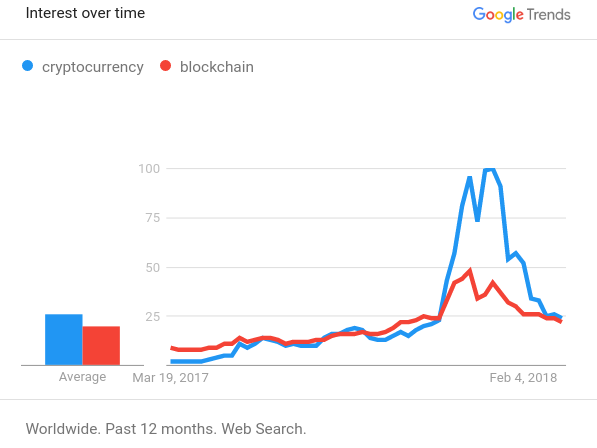
\includegraphics[width=\columnwidth]
{../images/trendscryptoblockchain.png}
  \caption{Google Trends: Cryptocurrency vs.
Blockchain~\cite{GoogleTrendsCrypto-Blockchain}}
\label{f:googletrendchart}
\end{figure}

The hype for cryptocurrency and blockchain technologies has led to major jumps
in various company stock prices who wither mention blockchain in a press
release or even toy with the name ``Bit'' or ``Block'' as a part of the company
name itself~\cite{ReutersKodak}. According to Gartner's Hype Cycle for Emerging
Technologies for 2017, blockchain is well within the ``Peak of Inflated
Technologies'' phase and therefore it will be some time before blockchain is
adopted as the game-changer technology behind the
hype~\cite{GartnerHypeTechnology2017}. More information on the technology
behind and concept of Blockchain can be found at
\textit{\url{https://www.ibm.com/developerworks/cloud/library/
cl-blockchain-basics-intro-bluemix-trs/}}.
Additionally, see Figure~\ref{f:blockchainpng} for a basic example of a
transaction on a blockchain.

\begin{figure}[!ht]
  \centering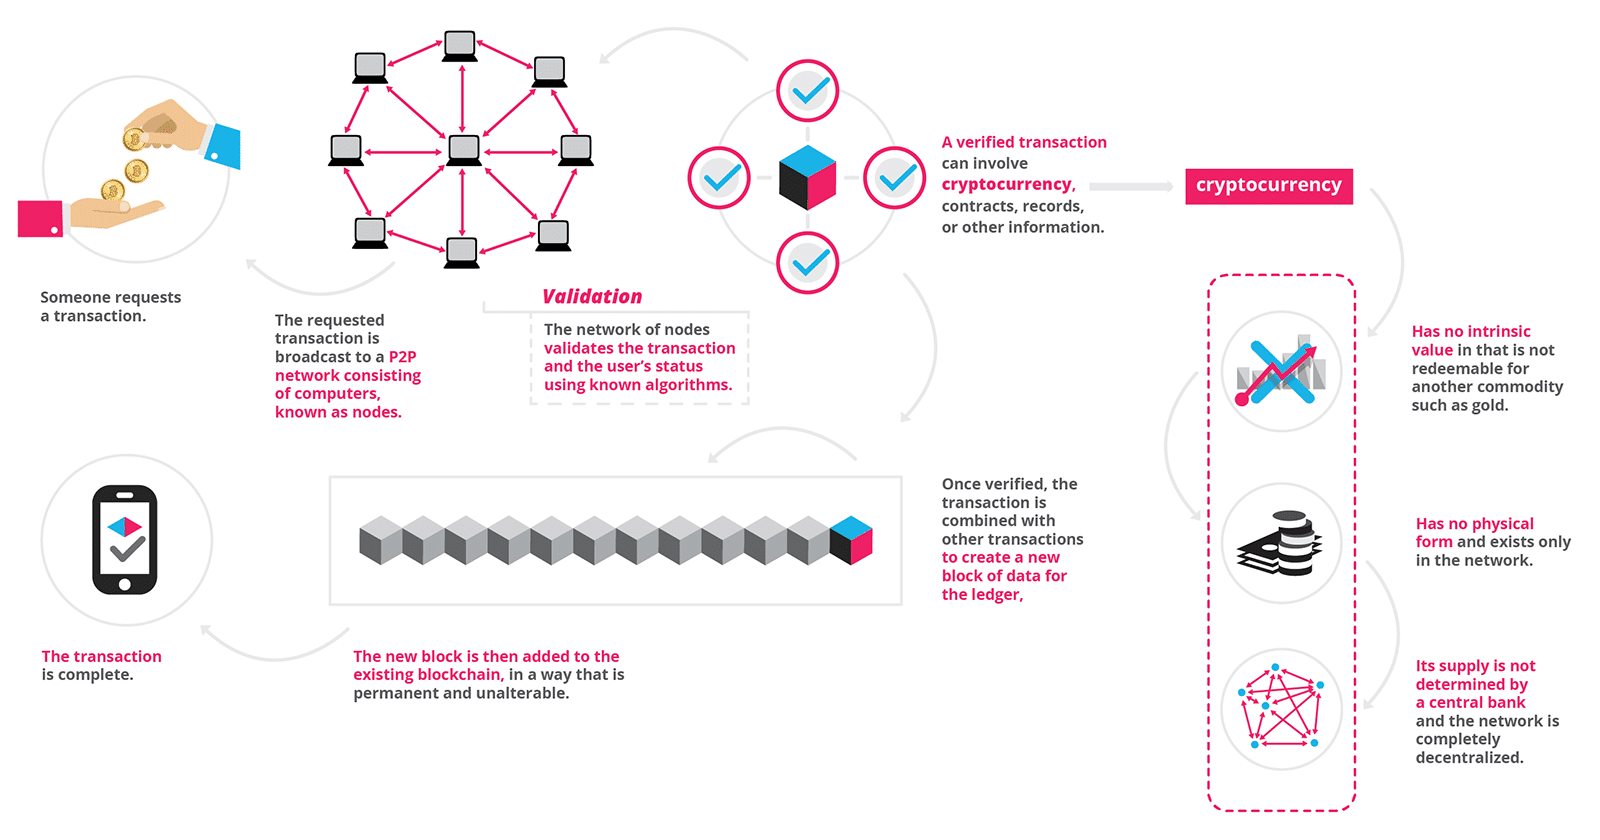
\includegraphics[width=\columnwidth]
{../images/blockchainbasics.png}
  \caption{Example Transaction on a Blockchain~\cite{BlockchainImage}}
\label{f:blockchainpng}
\end{figure}

\section{Openchain}
Openchain aims to narrow the time to enlightenment in using blockchain and the
Openchain technology enables developers, clients, consumers, and large
businesses to deploy and benefit from the open source blockchain capabilities
that are available already. Blockchain itself is traditionally implemented as a
distributed ledger where each node or entity on the connected network keeps a
copy of the ledger and through cryptography, anonymity, and the chain itself,
guarantees security and reliability in maintaining accurate, valid ledger
entries. One of the original and most famous implementations of the blockchain
technology is Bitcoin, a decentralized digital currency with a price determined
by the market for the currency itself. Bitcoin transactions, or the passing of
the digital coin from one owner to another is verified and maintained by the
blockchain so that no one ledger can claim  a false transaction compared to the
other ledgers on the chain. Early adopters of blockchain usages boast that in
order to fake a transaction or alter a transaction, the entirety of the chain
would need to be reverified and re-recorded; this implies that thousands of
nodes on a network would need to be changed instantly (a feat Don Tapscott, a
Co-Founder of the Blockchain Research Institue once described as ``turning a
Chicken McNugget back into a chicken''~\cite{DonTapscottPBS}), thus
guaranteeing security. However, this concept of wide distribution, although
secure, is not beneficial in a large-scaled environment. Bitcoin and other
instantiations of this early concept of peer-to-peer, distributed, anonymous
validation processes are often time consuming with verification times spanning
multiple days while the nodes sync in validation. Challenges such as this can
be solved by alternative blockchain technologies, such as the enterprise-ready
blockchain technology by Openchain~\cite{CoindeskCoinprism}.

Coinprism, the parent company to Openchain, and its founder, Flavien Charlon,
have pioneered multiple technologies utilizing blockchain concepts and
developed Openchain as a way for large industries to tailor a blockchain to its
own industry standards~\cite{BitcoinNewsOpenchain}. In a presentation with
CoinDesk, a leading cryptocurrency and blockchain news outlet, Charlon
explained that large industries and private companies saw the value in using a
blockchain to manage asset ownership but were hesitant to adopt blockchain
because of the increasingly longer validation cycles and veil behind not
knowing who is a part of validating or denying transactions on an open
chain~\cite{CoinDeskCharlonYouTube}. What makes Openchain a viable solution to
private industry concerns, beyond its ability to be deployed in seconds, is
that the private entity is the owner and administrator of all aspects of its
own blockchain ledger. This means that a company who manages the land leases of
thousands of lease contracts can enable its own third party resources to
validate contracts rather than relying on the potential for lease-expertise or
even competitors to approve transactions.

Openchain can function as a standalone blockchain, can be deployed beside other
closed blockchains, or be developed as a ``sidechain'' to other existing
blockchain technologies, such as a Bitcoin or Ethereum
chain~\cite{OpenchainHome}. The end-users of a chain can exchange the asset
freely within the openchain  per the rule and validation characteristics that
the administrator sets. Administrators can elect to have asset-specific
validating entities and can maintain multiple chains for each asset-type it
handles. For instance, the company that maintains a ledger for land-leases can
also administrate a ledger for the ownership of cars, gift-cards, medical
expense history, or even digital currencies, and can choose to combine the
chains to leave as individual standalone instances.

In addition to the blockchain technology designed for enterprise asset
management, Openchain offers a digital wallet, compatible with its openchain
technology so that the end-user can store the digitized asset and have any
transactions and ownership validated by the chain its connected to. Through
Openchain, a company, large or small, can implement and administer its own
private blockchain as well as provide a digital wallet for client use. This
model is common among small companies which use blockchain technologies and
private coins or tokens to fund projects as a means of venture capitalism
instead of the traditional and policy-laden concept of stocks through public
offerings.

\section{Under The Hood}
Under the hood of an Openchain server you'll see Openchain uses a Docker image
to set up the requirements and dependencies when spinning up the service. You
can build an Openchain instance without docker and the documentation is
provided by Openchain, although the configuration of both the docker-provided
setup and the self instantiation are identical. The server itself defaults to
using SQLite for the storage of transaction data, although you can use
SQLServer. Additionally, customization and support for development and
implementation are available via the active Openchain
forum~\cite{OpenchainForum}. Openchain is written in JavaScript and therefore
natively uses JSON formats for its HTTP API. The available methods include
POST, for submitting a transaction for validation, and GET, for retrieving
information of a validated transaction. Note, once a transaction is validated,
there is no way to append or adjust the ledger entry. The validation process
itself, via a POST method, involves submitting transaction data, which is
mutated via a hex-encoded byte string, and then hashing the mutation via double
SHA256~\cite{SHA256Wiki}. Finally, the transaction is signed using a
private-public key pair, of which the private key is signed using Secp256k1, a
popular cryptographic curve in blockchain signatures~\cite{Secp256k1Wiki}.

\section{Conclusion}
Despite the hype and the general population's misconceptions of blockchain,
Openchain offers a simple, yet powerful opportunity for organizations and
individuals to implement their own secure blockchain instance. Whether the
purpose is to handle the initial offering of a (hopefully) useful investment
currency, to backup personal digital assets, or to have a tangible back-story
to claims that your company is exploring blockchain technology so that your
public stock price soars, Openchain is available as an open source, highly
customizable, simple, and widely supported blockchain technology.

\bibliographystyle{ACM-Reference-Format}
\bibliography{report}
